\section{Introduction}
\subsection{Preface}
\label{cha:Goals}
With the improvement of computers we are able to tackle with high dimensional 
problems in control or pattern recognition task. At first glance everything
looks so easy, but when we go deeper into a problem more and more problems 
become evident and unavoidable. For example pattern can be described by many 
attributes. Some of them are very meaningful while others brings only noise 
and distortion. This is the role of the algorithm to pick valuable attributes,
but finding a minimal attribute reduct is $\mathcal{NP}$-hard problem. Another
obstacle is connected with overlaps in the attribute space. When attributes 
are easily separable even a simple classifier works perfectly, but for more 
tricky cases very sophisticated approaches have to be applied.

For the past years, many scientist in the world tried to invent new algorithms 
to improve the accuracy of classification or optimize control of the plant.
There are many solutions, but ones of the most eminent in the literature are: 
neural networks, fuzzy logic or evolutionary algorithms such as genetic algorithm. 
Because simple approaches failed in more complicated problem, scientist tried to applied 
algorithms for dimensionality reduction and merge abilities of single
classifier into combined one. This improved the quality of classification 
significantly, but until then no one has managed to invent such a classifier 
that will make no mistakes.

This thesis touches the broad topic of pattern recognition task which is 
very difficult and demanding problem in every aspect of science. Generally, 
pattern classification is about assigning label to an unknown object based 
on the available knowledge. It can be compared to the capability of human 
brain which is able to put certain scenario into context and identify 
distinguishable object components. The whole process of classification can 
be broken down into few parts and each phase has a significant impact on the
final results (more detailed description will be presented in \ref{cha:pattern
recognition}.

\subsection{Main goals of the  thesis}
This thesis concerns the problem of pattern recognition. As it was previously
said, in the literature one can find many algorithms used for object
classification, while here the rough sets and fuzzy logic algorithms are used 
and investigated. General purpose of this thesis is to propose hybrid
classifier using the power of fuzzy logic and rough sets. First of all the
mathematical background of these algorithms will be presented and later
simulation investigation will be carried out to prove the usefulness of
proposed fusion. It should be noted that for the simulation purposes author
implemented basic fuzzy logic, rough sets algorithms and created a hybrid
classifier.

This thesis is a continuation of work in the field of pattern recognition.
The results of previous experiments can be found in \cite{bib1}, \cite{bib2}. 
The aim of this paper is to collect all experiments scenarios in one place and draw
conclusions. It is meant to show the steps of constructing advanced hybrid
classifier from the basic algorithms. At first, the basic properties of rough
sets algorithm is checked in simulations, later the algorithm for 
modification decision rules is introduced and at the end as the final point
hybridization of algorithms is proposed.

At the end of this section, the experiment environment should be characterized in
few words. Given is the problem of pattern recognition (classification): in
this thesis datasets from $UCI$ Repository will be used (described in section
\ref{cha:experiment}. Those datasets are broadly available and everyone in the
future would be able to repeat the simulation investigation and compare the
results with those presented in this paper. To find is the algorithm classification accuracy on the given dataset.
Figure \ref{fig:input_output} shows the general schematic of the simulation
environment.
\begin{figure}[H]
    \begin{center}
        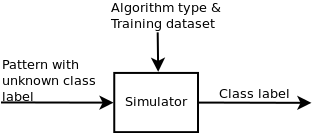
\includegraphics[width=\textwidth, height=0.5\textwidth]{fig/schema.png}
    \end{center}
    \caption{General schema of simulation environment. Input/output of the
    system}
    \label{fig:input_output}
\end{figure}

\subsection{Scope of this project}
This paper comprises of two parts. In the first, the review of
literature and the basic notation used in the whole paper is presented. Sections
\ref{cha:Introduction} is the source of the basic
knowledge about pattern recognition. Sections \ref{cha:Rough_set}, \ref{cha:Fuzzy_logic}
presents the description of algorithms used in this thesis. Additionally, this
part shows the algorithm construction steps using pseudo-code.

The second part, which is the main point of this thesis, presents experiments analysis.
Paragraph \ref{cha:ExperimentAnalysis} describes the experiment environment
setting and program written in $\mathcal{C++}$ to simulate standard sequential genetic
algorithm and its parallel counterparts. Results with comments are placed in
section \ref{cha:investigation}. Plans for the future work and general
conclusion are placed in sections \ref{cha:FutureWork}, \ref{cha:Summary}
respectively. 

